\section{Versuchsaufbau und Versuchsdurchführung}


\subsection{Bestimmung der Filterkurve des Selektiv-Verstärkers}

\begin{flushleft}
    Der Aufbau aus diesem Versuchsteil besteht aus einem Frequenzgenerator, einem Selektivverstärker, einem Voltmeter und zwei Kabeln.
    Das Voltmeter kann optional auch mit einem Oszilloskop gewechselt werden.
    Der Generator wird mit Selektivverstärker über ein Kabel verbunden und der Selektivverstärker mit dem Voltmeter an dem die Spannung angezeigt wird.
    Zusehen ist der Aufbau in Abbildung \ref{Abbildung4}. 
    Es werden etwa 40 verschieden Frequenzen eingestellt die in dem Intervall von $10\,\unit{\kilo\hertz}$ bis $35\,\unit{\kilo\hertz}$ auswählbar sind.
    Die Güte wird an dem Selektivverstärker auf 20 eingestellt und die Verstärkung auf 10fach gestellt.
\end{flushleft}

\begin{figure}[H]
    \centering
    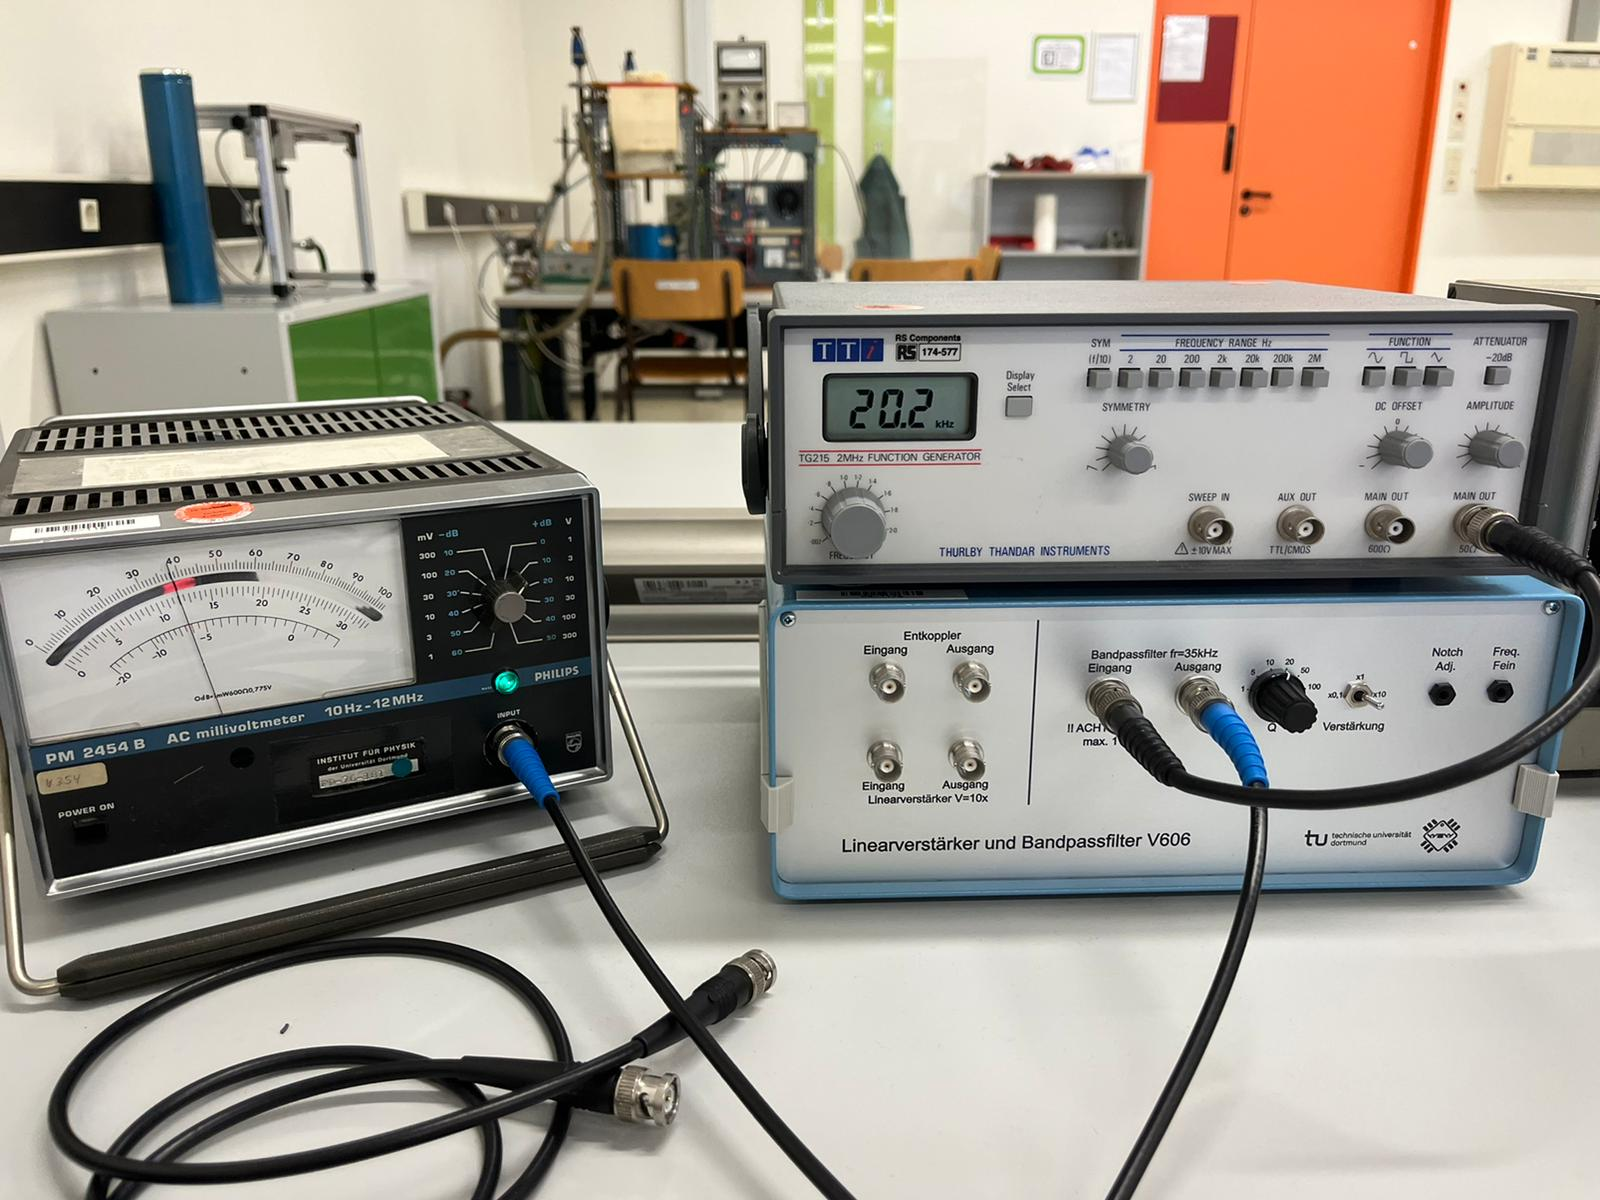
\includegraphics[height=60mm]{bilder/Ab4.jpeg}
    \caption{Der Aufbau der ersten Aufgabe.\label{Abbildung4} }
\end{figure}

\subsection{Bestimmung der Suszeptibilität}

\begin{flushleft}
    Der Aufbau aus diesem Versuchsteil besteht aus einem Sinus-Generator, der Brückenschaltung, einem Selektivverstärker, einem Voltmeter, drei verschiedenen Proben und Kabeln.
    Der Sinusgenerator wird mit dem Eingang für die Speisespannung verbunden, der Eingang der Brückenspannung wird mit dem Selektivverstärker verbunden und der Selektivverstärker mit dem Voltmeter.
    Zuerst wird die Brückenspannung auf null bzw. minimal gesetzt durch das variieren des Potentiometers und die Frequenz davon, sowie die Ziffer des Potentiometers aufgenommen.
    Danach wird in eine Spule eine Probe gegeben, die daraus entstehende Frequenz aufgenommen und die Brücke wieder abgeglichen. 
    Die Ziffer die das Potentiometer anzeigt nach dem messen wird ebenfalls notiert. 
    Durchgeführt wird dies für alle drei Proben jeweils drei mal.
\end{flushleft}

\begin{figure}[H]
    \centering
    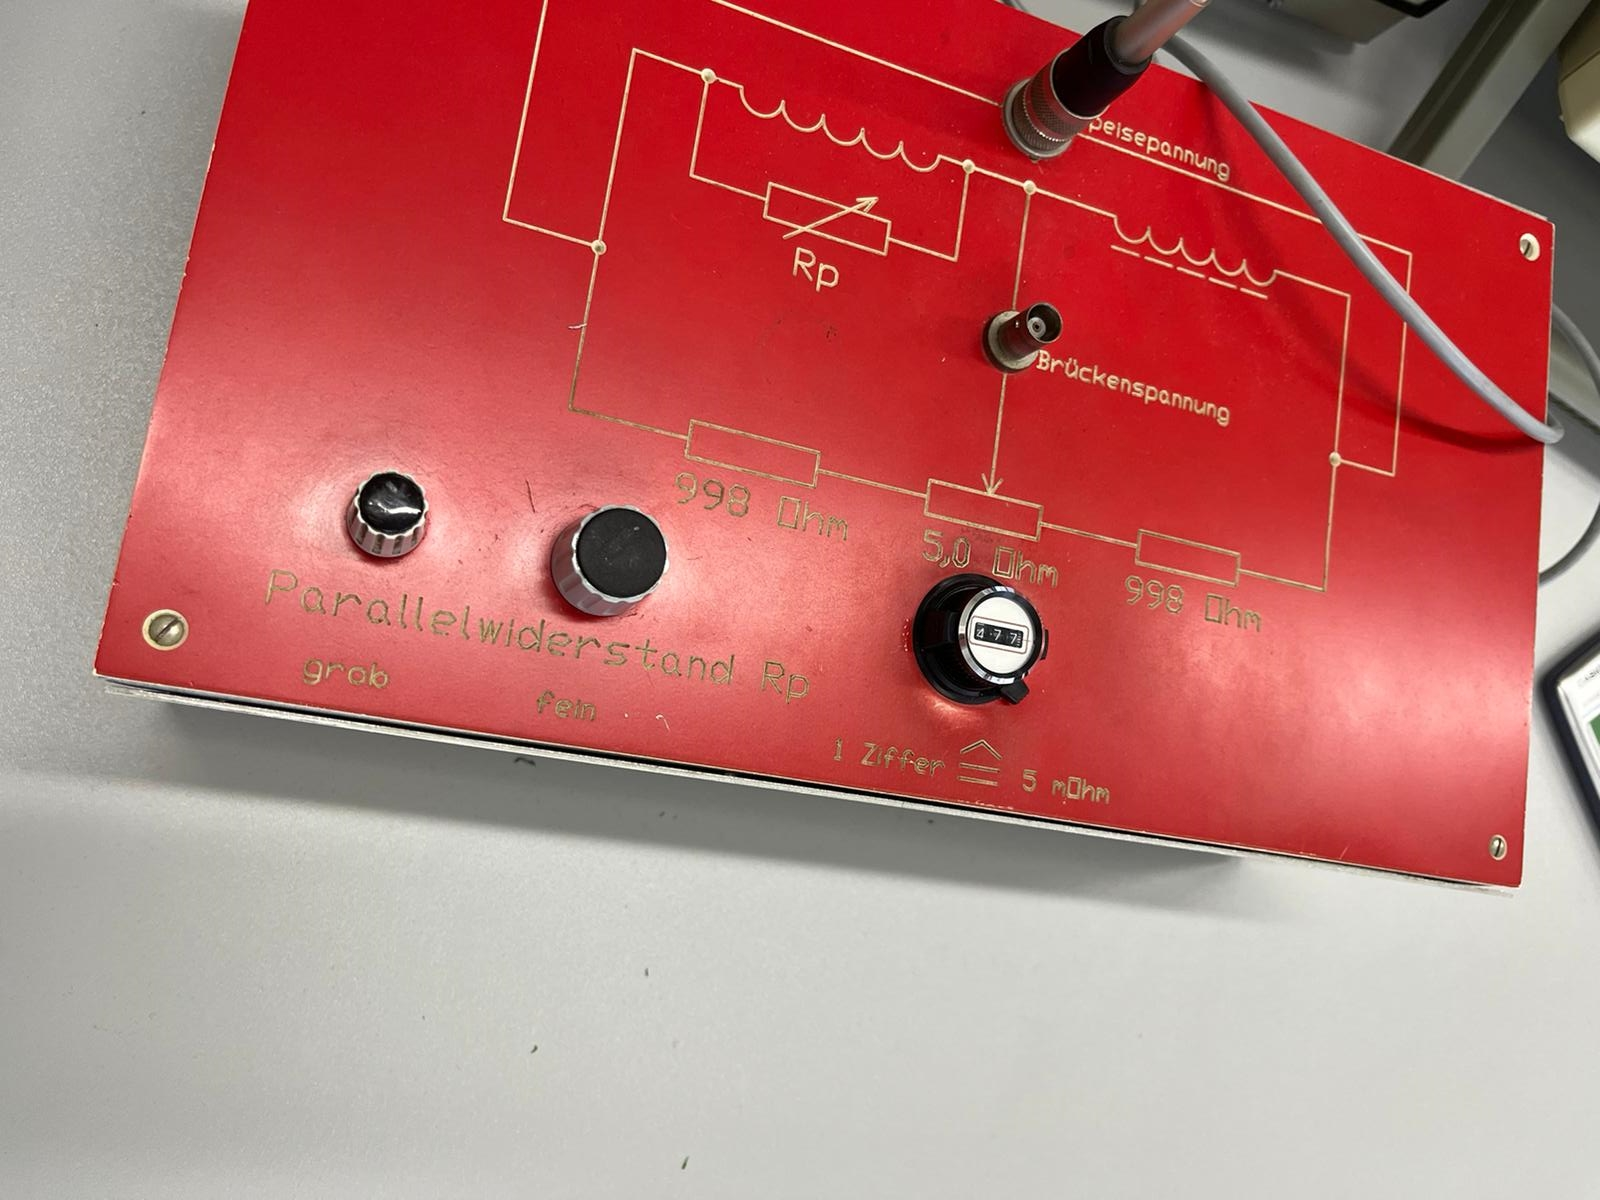
\includegraphics[height=70mm]{bilder/Ab5.jpeg}
    \caption{Abbildung der verwendeten Brückenschaltung.\label{Abbildung5} }
\end{figure}
